\documentclass[10pt,a4paper,twocolumn]{article}
\usepackage[T1]{fontenc}
\usepackage[utf8]{inputenc}
\usepackage{lmodern}
\usepackage[a4paper,textwidth=510pt,columnsep=18pt,top=1.9cm,bottom=2.2cm,hcentering]{geometry}
\usepackage{amsmath,amssymb,amsthm}
\usepackage{booktabs}
\usepackage{graphicx}
\graphicspath{{figures/}}
\usepackage{microtype}
\usepackage{bm}
\usepackage[font=small,labelfont=bf,skip=4pt]{caption}
\usepackage{titlesec}
\usepackage{xcolor}
\usepackage{placeins}
\usepackage[titles]{tocloft}
\setlength{\cftbeforesecskip}{5pt}
\setlength{\cftbeforesubsecskip}{1pt}
\usepackage[colorlinks=true,linkcolor=black,citecolor=black,urlcolor=blue!55!black]{hyperref}
\setlength{\emergencystretch}{2em}
\setlength{\parskip}{0pt}
\titlespacing*{\section}{0pt}{11pt plus 3pt minus 2pt}{5pt plus 1pt}
\titlespacing*{\subsection}{0pt}{8pt plus 2pt minus 2pt}{3pt plus 1pt}
\titleformat{\section}{\large\bfseries}{\thesection}{0.6em}{}
\titleformat{\subsection}{\normalsize\bfseries}{\thesubsection}{0.6em}{}
\setlength{\textfloatsep}{12pt plus 3pt minus 3pt}
\setlength{\dbltextfloatsep}{12pt plus 3pt minus 3pt}
\setlength{\floatsep}{10pt plus 3pt minus 2pt}
\renewcommand{\topfraction}{0.9}
\renewcommand{\dbltopfraction}{0.9}
\renewcommand{\textfraction}{0.08}
\renewcommand{\floatpagefraction}{0.8}
\renewcommand{\dblfloatpagefraction}{0.8}
\newtheorem{theorem}{Theorem}
\DeclareMathOperator{\rank}{rank}
\newcommand{\repourl}{https://github.com/HellWithCode0/layer-code-fault-tolerance}
\hypersetup{pdftitle={Universal Fault-Tolerant Computation on Three-Dimensional Layer Codes at Optimal Distance},pdfauthor={},pdfsubject={IRIS National Fair 2026 research paper}}
% Generated by hardware/hardware_summary.py; do not edit by hand.
\newcommand{\hwIQMwOne}{2.4}
\newcommand{\hwIQMwTwo}{0.070}
\newcommand{\hwIQMwThreeUpper}{0.033}
\newcommand{\hwIQMwThreeKept}{11{,}529}
\newcommand{\hwIQMctrl}{2.2 to 3.3}
\newcommand{\hwIQMpOneTwo}{\ensuremath{9.5\times10^{-19}}}
\newcommand{\hwIQMpTwoThree}{\ensuremath{0.071}}
\newcommand{\hwIBMwOne}{5.8}
\newcommand{\hwIBMwTwo}{0.59}
\newcommand{\hwIBMwThree}{0.14}
\newcommand{\hwIBMpOneTwo}{\ensuremath{1.7\times10^{-278}}}
\newcommand{\hwIBMpTwoThree}{\ensuremath{1.1\times10^{-16}}}
\newcommand{\hwIBMctrl}{7.2 to 7.9}
\newcommand{\hwMult}{0.53}
\newcommand{\hwMultCtrl}{2.3}
\newcommand{\hwMultP}{\ensuremath{5.1\times10^{-10}}}
\newcommand{\hwMultVsTwoP}{\ensuremath{0.0017}}
\newcommand{\hwRndIQMOne}{6.2}
\newcommand{\hwRndIQMTwo}{0.31}
\newcommand{\hwRndIQMModelOne}{6.9}
\newcommand{\hwRndIQMModelTwo}{0.34}
\newcommand{\hwRndIQMp}{\ensuremath{2.4\times10^{-188}}}
\newcommand{\hwRndIQMctrl}{7.7}
\newcommand{\hwRndIBMOne}{4.6}
\newcommand{\hwRndIBMTwo}{1.1}
\newcommand{\hwRndIBMThree}{0.59}
\newcommand{\hwRndIBMModelTwo}{0.18}
\newcommand{\hwRndIBMModelThree}{0.0086}
\newcommand{\hwPersSingle}{1.15}
\newcommand{\hwPersDouble}{1.11}
\newcommand{\hwPersIndep}{0.051}
\newcommand{\hwPersRatio}{23}
\newcommand{\hwPersRel}{3}
\newcommand{\hwPersP}{\ensuremath{8.8\times10^{-6}}}
\newcommand{\hwResetTwoS}{1.3}
\newcommand{\hwResetTwoD}{1.2}
\newcommand{\hwResetThreeS}{0.76}
\newcommand{\hwResetThreeD}{0.68}
\newcommand{\hwResetTwoP}{\ensuremath{0.15}}
\newcommand{\hwResetThreeP}{\ensuremath{1.8\times10^{-5}}}
\newcommand{\hwRndIBMpOneTwo}{\ensuremath{<10^{-300}}}
\newcommand{\hwRndIBMpTwoThree}{\ensuremath{<10^{-300}}}
\newcommand{\hwRndIBMmaxP}{\ensuremath{9.3\times10^{-123}}}
\newcommand{\hwRndIBMctrl}{4.3 to 4.4}
\newcommand{\hwFezCZ}{50, 55 and 60}
\newcommand{\hwQpuFez}{54}
\newcommand{\hwQpuA}{485}
\newcommand{\hwQpuB}{407}
\newcommand{\hwDecTwo}{3.0}
\newcommand{\hwDecThree}{1.7}
\newcommand{\hwDecP}{\ensuremath{6.4\times10^{-12}}}
\newcommand{\hwTotalShots}{6.9}
\newcommand{\hwStuck}{30{,}000}
\newcommand{\hwIQMfold}{35}
\newcommand{\hwIBMfoldOneTwo}{9.7}
\newcommand{\hwIBMfoldTwoThree}{4.3}
\newcommand{\hwMultFold}{4.6}
\newcommand{\hwRndIQMfold}{20}
\newcommand{\hwRndIBMModelRatio}{68}

\begin{document}

%======================================================================
% Title page
%======================================================================
\begin{titlepage}
\centering
\vspace*{1.6cm}
{\LARGE\bfseries Universal Fault-Tolerant Computation on\\[4pt]
Three-Dimensional Layer Codes at Optimal Distance\par}
\vspace{1cm}
{\large Research paper\par}
\vspace{0.35cm}
{\normalsize Category: Physics and Astronomy (PHYS)\qquad Individual project\par}
\vspace{1.3cm}
\begin{minipage}{0.8\textwidth}
\centerline{\bfseries Abstract}
\smallskip
Quantum computers must correct errors, and in three dimensions the layer codes
of Williamson and Baspin store quantum information at the highest density that
local checks allow.  Computing with them requires measuring their logical
operators locally, without losing that protection.  We give an
explicit lattice realization of the layer code for any CSS input code and prove
that every pure-$X$ logical operator has a representative on a single lattice
layer, at every height, and every pure-$Z$ logical operator one in a single
plane, built by a running (prefix) parity along each check.  These slabs are
measured by gauging with a nearest-neighbor three-dimensional grid of ancillas.
We prove that a grid with a constant number of ancillas per edge keeps the full
code distance, whereas any measurement layer of bounded thickness cannot,
because a thin interface contains a wall of few edges that a few faults can
cross.  With encoded resource transfer, distillation and a local detector
schedule, this gives a universal fault-tolerant architecture under
local-stochastic Pauli noise with the optimal distance $\Theta(N^2)$ and
$O(Wf+f^{3/2})$ physical qubits for $W$ logical sites.  Circuit-level
simulations of joint measurements on explicit layer-code blocks (up to
$16{,}293$ qubits) confirm the contrast between thin and thick interfaces.  On
IQM and IBM superconducting processors (\hwTotalShots~million samples), widening
the interface from one edge to two lowers the measurement error
\hwIQMfold-fold and \hwIBMfoldOneTwo-fold respectively, and repeated rounds
protect the reported bit, except where ancilla errors survive a reset, a failure
mode outside the noise model.

\medskip
\noindent\textbf{Keywords:} quantum error correction; layer codes;
fault-tolerant quantum computation; logical measurement; gauging;
superconducting qubits.
\end{minipage}
\vfill
\end{titlepage}

%======================================================================
% Contents and key terms
%======================================================================
\onecolumn
\setcounter{page}{2}
\tableofcontents

\vspace{1cm}
\noindent\textbf{\large Key terms used in this paper}
\medskip

\noindent
\begin{tabular}{@{}p{0.2\textwidth}p{0.77\textwidth}@{}}
\toprule
Qubit & A two-level quantum system; \emph{physical} qubits are the hardware, \emph{logical} qubits the protected information they encode.\\
Stabilizer (check) & A product of Pauli operators ($X$, $Z$) whose measured value is fixed when there is no error; a changed value reveals an error.\\
CSS code & A code whose checks are all of $X$ type or all of $Z$ type, so that $X$ and $Z$ errors are caught separately.\\
$[[n,K,d]]$ & A code with $n$ physical qubits, $K$ logical qubits and distance $d$.\\
Distance $d$ & The smallest number of physical errors that changes the logical information without changing any check.\\
Fault distance & The smallest number of faults (gate, idle or measurement errors) in a whole circuit that cause an undetected logical error.\\
Logical operator & An operator that acts on the logical qubits and commutes with every check; its \emph{representatives} differ by checks.\\
Ancilla & An extra qubit used to measure a check or a logical operator.\\
Gauging & Measuring a logical operator as the product of many small local checks on an added ancilla grid.\\
Wall & A set of grid edges whose removal separates the ports of one block from those of the other.\\
Detector & A parity of measurement outcomes that is fixed without noise; postselection keeps only samples in which every detector is silent.\\
LDPC & Low-density parity check: every check acts on a bounded number of qubits, and every qubit is in a bounded number of checks.\\
$\Theta$, $O$, $\Omega$ &``Proportional to'', ``at most proportional to'' and ``at least proportional to'', for large sizes.\\
\bottomrule
\end{tabular}

\twocolumn
%======================================================================
\section{Introduction}
\label{sec:intro}
%======================================================================
\subsection{Why quantum computers need local error correction}
Quantum bits lose their information quickly through noise, so a large quantum
computer must correct errors faster than they accumulate.  A quantum
error-correcting code stores $K$ logical qubits in $n$ physical qubits and
repeatedly measures parity checks that reveal errors without disturbing the
stored information.  Its distance $d$ is the smallest number of physical errors
that can change the stored information unnoticed, so a code of large $d$
tolerates many errors.

Real devices also need \emph{geometric locality}: every check and gate should
involve only nearby qubits.  Locality limits what a code can do.  In three
dimensions every local stabilizer code obeys $Kd=O(n)$ \cite{BPT}, so
$\Theta(d)$ physical qubits per logical qubit is the best possible storage
cost.  Surface-code patches processed by lattice surgery, today's standard, use
$\Theta(d^2)$ \cite{HorsmanLatticeSurgery,LitinskiSurgery}, and
three-dimensional surface and color codes trade larger volume for transversal
gates \cite{VasmerBrowne}.  The layer codes of Williamson and Baspin
\cite{WilliamsonBaspinLayerCodes} reach the limit.  They embed a CSS code into a
local network of surface-code sheets and defects; for balanced good
low-density parity-check (LDPC) inputs of length $N$, the blocks have
\begin{equation}
 n=\Theta(N^3),\qquad K=\Theta(N),\qquad d=\Theta(N^2),
 \label{eq:parameters}
\end{equation}
with bounded-weight, geometrically local checks.

\subsection{The problem: storage is not computation}
A memory is useful only if it can also compute.  For codes of this kind,
computation is done by measuring logical Pauli operators, for example the joint
parity $\overline X_a\overline X_b$ of logical qubits in two blocks, through an
added system of ancilla qubits
\cite{WilliamsonYoderGauging,CowtanParallelSurgery,IdeHomological}.  Two
obstacles appear for layer codes.  A logical operator of a layer code is spread
through the whole block, and general measurement schemes for LDPC codes need
ancilla graphs with expander properties, which are not local in three
dimensions.  Moreover, adding measurement layers to a layer code can, in
principle, reduce its distance, so the optimal storage could be lost exactly
when the code is used.

\subsection{Research question, objectives and hypothesis}
\textbf{Research question.} Can a three-dimensional layer code perform
universal, fault-tolerant quantum computation with nearest-neighbor operations
only, while keeping its optimal distance $d=\Theta(N^2)$?

\begin{enumerate}
\item[(O1)] Build an explicit, checkable lattice for the layer code and find
representatives of its logical operators that occupy a single thin layer.
\item[(O2)] Design a local logical measurement that keeps the full distance,
and identify which measurement interfaces lose it.
\item[(O3)] Combine these measurements into a universal fault-tolerant
architecture and compute its cost in qubits and time.
\item[(O4)] Test the distance mechanisms in circuit-level simulations of
explicit layer-code blocks and on superconducting quantum processors.
\end{enumerate}

\noindent\textbf{Hypothesis for (O4).} The fault distance of a joint logical
measurement is limited by the smallest wall of interface edges between the two
blocks.  Hence its error should fall sharply when the interface is widened,
when parallel ancillas are placed on an interface edge, and when the
measurement is repeated over more rounds.

\subsection{Background and related work}
Logical measurement by gauging, surgery and homological constructions has
become a general route to processing quantum LDPC codes
\cite{WilliamsonYoderGauging,CowtanParallelSurgery,YuanParsimonious2026,IdeHomological,BerentLiftedSurgery}.
Adapters, extractors and universal architectures address complementary
questions of connectivity, parallelism and resource overhead
\cite{SwaroopAdapters,HeExtractors,ZhangGoodQLDPC,MalcolmEfficientQLDPC}.
Local simulations of LDPC codes \cite{PattisonHierarchical}, local
fault-tolerance constructions \cite{ChoeKoenigLocal}, wire codes
\cite{BaspinWire} and planar logical measurements \cite{YangPlanar} address
related geometric questions, while constant-overhead schemes
\cite{GottesmanFTThreshold,KovalevPryadko,FawziGrospellierLeverrier} and LDPC
magic-state injection \cite{ZhangInjectionIndependence,LiuInSituInjection} rely
on nonlocal connectivity.  Williamson and Baspin already obtain the layer-code
logical operators by quasi-concatenating input logicals
\cite{WilliamsonBaspinLayerCodes}.  What was missing is a representative that is
thin and movable, and a local measurement that provably keeps the distance.
Here the organizing constraint is three-dimensional Euclidean locality: logical
access, resource delivery and syndrome extraction all use the same
nearest-neighbor geometry.

\subsection{Contributions of this work}
\begin{itemize}
\item An explicit lattice realization of the layer code for any CSS input whose
checks have weight at least two, with a proof that it encodes exactly the input
logical qubits and that every pure-$X$ (pure-$Z$) logical operator has a
representative on a single lattice layer (plane) at every height (position).
These \emph{slabs} give the optimal distance $\Theta(N^2)$ for good inputs
(Theorem~\ref{thm:slabs}).
\item A local measurement of the slabs by three-dimensional grid gauging, which
keeps the full distance with a constant number of ancillas per edge, and a proof
that every measurement layer of bounded thickness loses distance (the
\emph{cut obstruction}).
\item A universal fault-tolerant architecture using $O(Wf+f^{3/2})$ physical
qubits for $W$ logical sites (Theorem~\ref{thm:architecture}), with a concrete
resource estimate and two structural bounds.
\item Circuit-level simulations of a complete joint logical measurement on
explicit layer-code blocks, with exact fault distances.
\item Demonstrations of the three distance mechanisms on IQM and IBM
superconducting processors, which also expose ancilla errors that survive a
reset, a failure mode outside the noise model of the theorem.
\end{itemize}

%======================================================================
\section{Methodology}
\label{sec:methods}
%======================================================================
\subsection{Approach}
The work combines three methods.  Mathematical proofs give the results for every
block size.  Computer certificates and circuit-level simulations test the
constructions on explicit finite blocks, including exact minimum-fault
calculations.  Hardware experiments test the distance mechanisms, which already
act in circuits small enough for present processors.
Figure~\ref{fig:overview} shows the architecture that the proofs build.  The
argument has three steps: a prefix-parity construction produces the slab
representatives (Sec.~\ref{sec:slabs}); relative expansion of a cubic grid
gives a local gauging measurement that keeps the distance
(Sec.~\ref{sec:distance}); and repeated extraction, padded composition and
encoded resource transfer give a complete circuit
(Secs.~\ref{sec:gates} to~\ref{sec:architecture}).

\begin{figure*}[t]
\centering
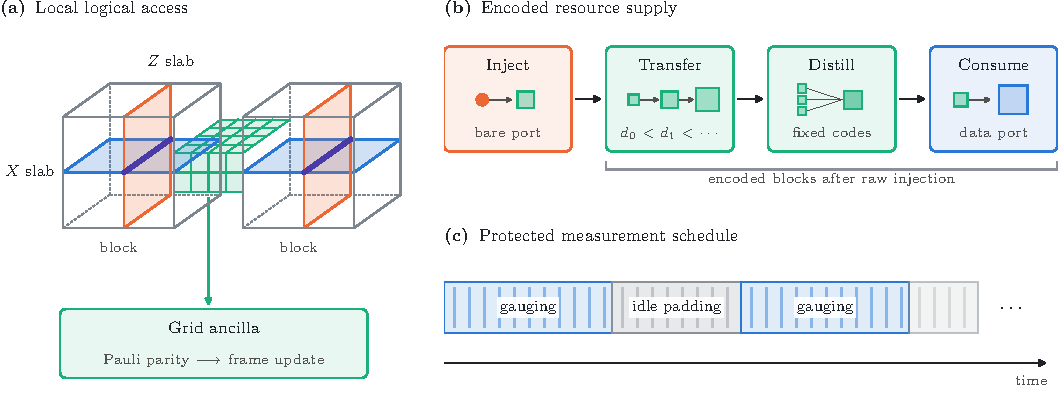
\includegraphics[width=\textwidth]{revision_architecture.pdf}
\caption{The architecture. (a) A layer-code block exposes single-layer slab
ports for pure-$X$ (blue) and pure-$Z$ (orange) logical operators.  A local grid
ancilla (green) measures the selected Pauli operator; neighboring blocks use the
same interface for joint measurements.  (b) A raw resource state is injected
into an encoded block, transferred through blocks of increasing distance,
distilled, and consumed by the data.  (c) Repeated extraction and idle padding
separate successive measurements.  All drawings are schematic; the encoded
blocks and grid ancillas occupy three-dimensional regions.}
\label{fig:overview}
\end{figure*}

\subsection{The layer code as glued surface-code sheets}
\label{sec:sheets}
A layer code is assembled from surface-code sheets
\cite{WilliamsonBaspinLayerCodes}.  Each qubit $q$ of the input CSS code becomes
a \emph{data sheet}, the plane $y=Y_q$; each input $Z$ check becomes a
\emph{$Z$-check sheet}, a plane $x=\mathrm{const}$; and each input $X$ check
becomes an \emph{$X$-check sheet}, a plane $z=\mathrm{const}$.  Every sheet is
an ordinary surface code on a rectangle of the cubic lattice, so it carries
string operators.  A string of $X$ operators that runs from one side of a sheet
to the other commutes with all checks of that sheet; a string that stops inside
the sheet leaves a violated check, a \emph{defect}, at its end.  A $Z$-check
sheet meets the data sheets of the qubits in its check along vertical lines,
the \emph{junctions}.  Ordered along the check, these are its first, middle and
last junctions.  The $X$-check sheets are attached in the same way, with $X$ and
$Z$ exchanged.

A junction is a rule that says which strings may end on the line without leaving
a defect.  At a first or last junction the $Z$-check sheet ends on the data
sheet, and the check-sheet string is present exactly when the data string is.
At a middle junction three strings meet the line: the data string, which
crosses it, and the check-sheet strings on its two sides.  They leave no defect
exactly when an even number of the three is present.  Writing $1$ for a present
string, and listing the check-sheet strings first and the data string last,
\begin{align}
 H_{\rm end}&=\begin{bmatrix}1&1\end{bmatrix}, &
 \ker H_{\rm end}&=\{00,11\},\nonumber\\
 H_{\rm mid}&=\begin{bmatrix}1&1&1\end{bmatrix}, &
 \ker H_{\rm mid}&=\{000,110,101,011\}.
 \label{eq:boundary}
\end{align}
Williamson and Baspin state these rules as sets of condensed anyons;
Eq.~\eqref{eq:boundary} is the same information written for $X$ strings.  The
word $110$ is the important one.  It lets a string on the check sheet pass a
data sheet without any string on that data sheet.  If a middle junction allowed
only $000$ and $111$, every check-sheet string would drag a string onto each
data sheet it passes, and the lattice would in fact fail to encode the input
qubits, as our certificate confirms.

We build every junction explicitly on the lattice.  Sheets own distinct qubits,
and each junction rule adds one qubit of one sheet to one check of the other.
At a middle junction the $Z$-check-sheet face beside the line gains the data
sheet's edge on the line.  That face then contains the check-sheet edge on the
line, where the string from one side ends; the next check-sheet edge, where the
string on the other side begins; and the added data edge.  Its check is
therefore exactly the middle rule of Eq.~\eqref{eq:boundary}.  The data stars on
the line gain the check sheet's edges on the same side, which keeps them
commuting with the modified faces.  At a first or last junction the check sheet
ends on the data line and shares its edges, which gives the two-bit rule.

One more repair is needed.  An $X$-check sheet and a $Z$-check sheet cross along
a line, and there the junction additions of the two sheets make a few stars and
faces anticommute, once for each data qubit shared by the two input checks.  A
row of one-qubit additions along the crossing line, which we call a
\emph{lattice wall}, removes these conflicts.  It exists exactly when the shared
number is even, which is the commutation of the two input checks.  The slab
operators below never use lattice-wall qubits.  Every check lies within unit
distance of one lattice vertex and has weight at most six.  The junctions have
the condensed anyons of Ref.~\cite{WilliamsonBaspinLayerCodes}; we do not claim
that the lattice is identical to the drawings there, and every result below is
proved for this explicit lattice, whose complete check matrices the script
\texttt{layer\_code\_explicit.py} in the project repository \cite{Repo}
generates.

\subsection{Logical measurement by gauging}
\label{sec:gauging}
Gauging measures a logical operator by measuring many small checks whose
product is that operator \cite{WilliamsonYoderGauging}.  Let $\overline P=X(D)$
be the selected logical representative.  Attach each data qubit of $D$ to its
own vertex of a connected grid $G=(V,E)$, call these vertices the \emph{ports}
$U$, and place an ancilla qubit on every edge.  The new check at a vertex, its
\emph{vertex star}, is $X$ on the edges at that vertex and on the attached data
qubit, if any.  Every edge belongs to two vertex stars, so the product of all
vertex stars is $\overline P$, and the product of their measured outcomes is the
logical outcome; yet each measurement involves only a few neighboring qubits.
The grid also carries $Z$ checks around its unit squares, and every original $Z$
check that meets $D$ is extended along short grid paths joining its ports, so
that it commutes with the stars.  Preparing the edge qubits in $|0\rangle$,
measuring the new checks for $R$ rounds, and finally reading the edges in $Z$
returns the data to its original code with an updated Pauli frame.  The
$X/Z$-exchanged construction measures pure-$Z$ logicals.

The danger is that the added qubits create new, shorter logical operators.  The
quantity that controls this is the expansion of the grid relative to its ports,
\begin{equation}
 \beta(G,U)=\min_{S\subseteq V}
 \frac{|\delta S|}{\min\{|S\cap U|,|U\setminus S|\}},
 \label{eq:beta}
\end{equation}
where $\delta S$ is the set of edges leaving $S$ and only positive denominators
are included.  We call $\delta S$ a \emph{wall}: it separates the ports in $S$
from the others, and $\beta$ is the smallest number of wall edges paid per port
separated.

\subsection{Noise model and fault distance}
\label{sec:noise}
We consider local-stochastic Pauli circuit noise: any specified set $F_0$ of
fault mechanisms at distinct locations occurs with probability at most
$p^{|F_0|}$; no independence is assumed.  A round of check measurements has
constant depth and uses only nearest-neighbor gates on a finite ancilla
schedule.  Each circuit fault acts like at most $c_1=O(1)$ elementary faults of
the simpler phenomenological model, in which a fault is a data error or a wrong
measurement outcome; we count faults in that model and divide by $c_1$ at the
end.  The \emph{fault distance} of a circuit is the smallest number of faults
that flips a protected outcome while leaving every detector silent.  For finite
circuits we compute it exactly: the script \texttt{min\_weight\_logical.py}
builds the detector error model of a circuit with Stim \cite{Stim} and finds the
smallest undetectable logical fault set with the CP-SAT solver of OR-Tools
\cite{CPSAT}.

\subsection{Circuit-level simulations}
\label{sec:sim-methods}
\textbf{Joint measurement on layer-code blocks.}  Each block is the explicit
realization of the $[[4,2,2]]$ input at lattice spacing $s=2,3,4,5$ ($n=224$,
$504$, $896$ and $1400$ qubits; $d_X=2s+1$, $d_Z=2s$).  Logical qubit~1 of two
blocks is measured jointly, $\overline X_1^{(a)}\overline X_1^{(b)}$, by gauging
on a grid attached to their single-layer slabs; logical qubit~2 of each block is
a spectator.  Each logical qubit starts maximally entangled with a noiseless
reference qubit, and eight observables test the output state, so the test covers
the reported bit, both logical sectors, the spectators and an entangled input.
Every check is measured with its own ancilla for $R=2s+1$ rounds before, during
and after the measurement.  The interfaces are a bridge of $w=1,2,3$ grid rows
between the blocks, a grid spanning both blocks (one or two ancillas per edge),
and, as a baseline, the same blocks left idle.

The noise is uniform circuit noise of strength $p$ from $0.5\times10^{-3}$ to
$6\times10^{-3}$: two-qubit depolarizing noise after every CNOT, one-qubit
depolarizing noise on every data and edge qubit in every round, and flips at
every reset and measurement, including the final data readout.  Each CSS sector
is decoded by belief propagation with localized statistics decoding (BP+LSD)
\cite{LSD}.  A paired comparison on identical shots shows that this decoder is
pessimistic for the grid, by up to a factor of two, and nearly matches the
full-model decoder for the bridge, so the contrast reported below is, if
anything, understated.  Each point ran until $200$ failures, a shot cap or the
end of a time budget, for $3.0\times10^6$ shots and $237$ core-hours in total,
in batches with recorded seeds; error bars are Wilson 95\% intervals
\cite{Wilson}.

\textbf{Routed circuits.}  A second set of circuits replaces the per-check
ancillas by a routed nearest-neighbor schedule: each ancilla moves by SWAP gates
along a spanning tree of reserved routing sites, overlapping checks run in
separate color classes, and every waiting qubit suffers idle noise in every time
step.  It grows the input at $s=2$, from $[[4,2,2]]$ to a six-qubit band code and
the Steane code $[[7,1,3]]$ ($n=224$, $720$ and $1792$; circuits of up to
$16{,}293$ qubits), and reports noiseless certification and exact fault
distances.

\textbf{Surface-code gauging campaign.}  A planar surface code of distance $L$
passes through a base-code $\to$ gauged-strip $\to$ base-code circuit, without
resetting the data between stages, under an SI1000-like model (two-qubit
depolarizing strength $p$, single-qubit and idle strength $p/10$, measurement
flips $5p$, reset noise $2p$).  The campaign comprises 255 parameter points and
$4.534\times10^6$ shots for $L=3,5,7,9,11$ and gauged durations $G=d,2d,3d$,
decoded by minimum-weight perfect matching \cite{PyMatching}.  It tests the
detector bookkeeping of a code switch, not the layer-code geometry.

\subsection{Hardware experiments}
\label{sec:hw-methods}
\textbf{Devices.}  We used the 54-qubit IQM Emerald processor (square lattice)
through the Open Quantum platform \cite{OpenQuantum2026}, with qubit rewiring
disabled, and the 156-qubit IBM Heron processors \texttt{ibm\_fez} and
\texttt{ibm\_kingston} (heavy-hex lattice) through the IBM Quantum Platform with
Qiskit \cite{Qiskit}, using \hwQpuFez~s, \hwQpuA~s and \hwQpuB~s of processor
time.  The data were taken on 13 and 14 October 2026.  The blocks are three-qubit
repetition codes, not layer codes, so the runs test the distance mechanisms,
not the architecture.

\textbf{Circuits.}  (i)~\emph{Cut obstruction.}  Two blocks with checks
$Z_0Z_1$, $Z_1Z_2$ and $\overline X=X_0X_1X_2$ start in $|000\rangle$, and
$\overline X_a\overline X_b$ is measured by gauging on a graph whose bridge
between the blocks has $w=1,2,3$ edges.  Each vertex star is measured once by
its own ancilla, read at the end, so no mid-circuit measurement is needed.  The
deformed $\overline Z_a\overline Z_b$ must read $+1$.  The detectors are the
deformed $Z$ checks and, for $w\ge2$, the cycle checks of the bridge squares;
$X$ on the $w$ bridge edges is a logical operator, so the exact circuit fault
distance is $w$.  On IQM the circuits use $16$, $18$ and $20$ CZ gates; routed
on \texttt{ibm\_fez} they need \hwFezCZ.  (ii)~\emph{Parallel ancillas.}  The
single bridge edge carries two ancillas, which adds the check $Z_eZ_{e'}$ and
raises the distance to two.  (iii)~\emph{Repeated rounds.}  Two phase-flip
blocks ($d_Z=3$) joined by one edge measure their two vertex stars and four block
checks in $R$ rounds; the reported bit is the product of the stars, and its
exact circuit fault distance is $\min\{R,3\}$.  On IQM, which does not allow a
measured qubit to be reused, every round uses fresh ancillas ($R=1,2$); on
\texttt{ibm\_kingston} the ancillas are measured and reset between rounds
($R=1,2,3$; run~B also tests two resets between rounds).

\textbf{Placement and checks.}  Apart from the routed \texttt{ibm\_fez}
circuits, every two-qubit gate acts on a physical coupler, so the circuits
contain no SWAP gate; the IQM placements are SWAP-free under both possible qubit
numberings of the platform.  On IBM the repeated-rounds layout was chosen from
the live calibration.  Before submission each circuit as sent was checked to
equal the reference circuit, to pass every detector without noise, and to have
the stated exact circuit fault distance.

\textbf{Analysis.}  Each result is the error of the observable after
postselection on every detector, with Wilson 95\% intervals; comparisons use
one-sided Fisher exact tests \cite{Fisher}.  As a control, the same samples are
reanalyzed with the checks that the better interface adds ignored.  For the
later runs the test and its level $0.05$ were fixed in the analysis script
before the jobs were submitted; for the first runs the analysis code was fixed
before the data, but the tests were chosen afterwards.  The bit order of each
output was verified from the data wherever possible.  Predictions come from
Pauli noise models with the devices' error rates.  Two attempts on a Rigetti
processor were excluded because most of their detectors fired at random (in the
second, one qubit read 1 in all \hwStuck{} shots although it was listed as
working); their outputs are archived.

%======================================================================
\section{Results}
\label{sec:results}
%======================================================================
\subsection{Logical operators in single-layer slabs}
\label{sec:slabs}
\begin{theorem}[Uniform slab representatives]
\label{thm:slabs}
For every input CSS code with checks of weight at least two, the explicit
realization encodes exactly $K$ logical qubits.  Every pure-$X$ logical class
has a representative supported on the single layer of $z$-edges spanning
$[z_0,z_0+1]$, for every height $z_0$ of the block, and every pure-$Z$ class has
a representative in the plane $x=x_0$, for every $x_0$.  The heights and planes
are chosen independently of the logical classes.
\end{theorem}

\begin{figure*}[t]
\centering
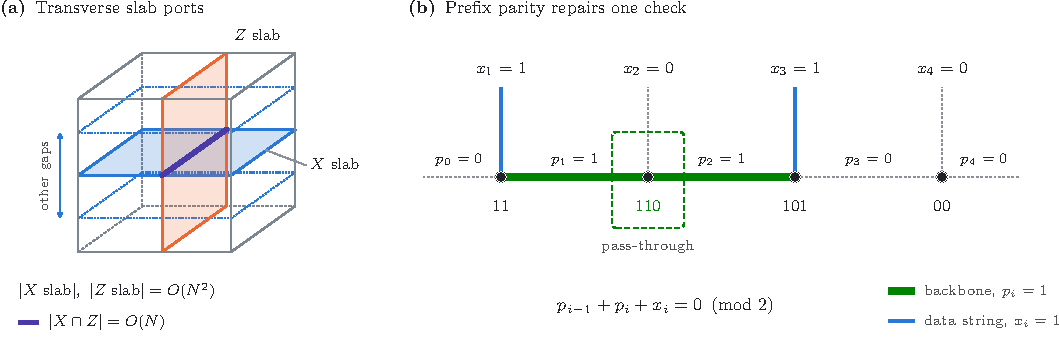
\includegraphics[width=\textwidth]{revision_slab_prefix.pdf}
\caption{Slab representatives and the prefix parity. (a) Complete $X$ and $Z$
ports occupy single-layer slabs.  Each slab contains $O(N^2)$ qubits, and two
crossing slabs share $O(N)$.  Translating a slab to another height (or plane)
gives another representative of the same logical class.  (b) For the incidence
word $(1,0,1,0)$ the running parity is $(0,1,1,0,0)$.  The highlighted middle
cell uses the word $110$: the backbone stays on although the data string is
absent.  End cells use the two-bit rule of Eq.~\eqref{eq:boundary}.}
\label{fig:slab-prefix}
\end{figure*}

\textbf{Construction.}  The operator is built at one fixed height $z_0$, one
input check at a time.  Choose a pure-$X$ logical $x\in\ker H_Z$ of the input
code and put an $X$ string at height $z_0$ on the data sheet of every qubit with
$x_q=1$.  Each string crosses the junction of every $Z$-check sheet attached to
its data sheet and, alone, would leave a defect there.  Along one $Z$-check sheet
the selected junctions must therefore be joined in pairs by strings on the check
sheet at the same height, which we call the \emph{backbone}.  Pairing is
possible because $x$ commutes with the input check, so the check contains an
even number of selected qubits.  Walk along the check from its first qubit and
switch the backbone at every selected junction.  With ordered incidences
$x_1,\ldots,x_k$, the backbone after the $i$th junction is present exactly when
an odd number of selected qubits lies behind it, a running count that we call
the \emph{prefix parity},
\begin{equation}
 p_0=0,\qquad p_i=\sum_{h=1}^{i}x_h,\qquad p_k=0,
 \label{eq:prefix}
\end{equation}
where $p_k=0$ is the commutation $\sum_ix_i=0$ over $\mathbb F_2$.  At every
middle junction $p_{i-1}+p_i+x_i=0$, so none or two of the three strings are
present, as Eq.~\eqref{eq:boundary} requires; at the ends $p_1=x_1$ and
$p_{k-1}=x_k$.  No defect remains anywhere (Fig.~\ref{fig:slab-prefix}).  Every
piece lies in the same layer of vertical edges, so the operator is one lattice
layer thick, whatever the block size and whichever logical is chosen.  Building
it at another height gives another representative of the same class.  In the
explicit realization the check is exact and local: every stabilizer meets the
operator in one of the forms $x_1+p_1$, $p_{i-1}+p_i+x_i$, $p_{k-1}+x_k$ of a
single incidence, or not at all.

\textbf{Exactly $K$ logical qubits.}  The pure-$Z$ operators are built in the
same way in a vertical plane $x=x_0$, with backbones on the $X$-check sheets.  An
$X$ slab operator and a $Z$ slab operator share only one data edge for each
input qubit selected by both, so they anticommute exactly when the two input
logicals do.  This gives $K$ independent logical qubits.  A count shows that
there are no others.  On its own, each data sheet would encode one qubit and
each check sheet would remove one; the junctions and lattice walls add neither
qubits nor checks; and every redundancy among the lattice checks comes from a
redundancy among the input checks.  Hence the realization encodes exactly $K$
qubits, and the slab operators represent every pure-type class.  A certificate
on complete codes with up to $10{,}936$ qubits, including the linear forms above
and exhaustive negative controls, checks each step.

\textbf{Distance.}  The same ports give the distance, by a simple idea: a
logical operator must be visible in every plane that contains a complete port of
the other type.  Let $O$ be a nontrivial $X$ logical.  It anticommutes with some
$Z$ logical, which has a slab representative in each of the $L_x+1$ disjoint
planes $x=x_0$, so $O$ must place qubits in every one of these planes.  Cut the
$Z$ slabs of one plane into pieces, a data column for each input qubit and the
backbone segments, and record which pieces $O$ meets an odd number of times.
Read as input qubits, the records spell out a nontrivial $X$ logical of the
input code, with at least $d_X^{\rm in}$ entries.  A backbone piece stands for
at most $\eta_X=\max\{1,\lfloor w_X/2\rfloor\}$ input qubits, where $w_X$ is the
largest input $X$-check weight, because the first $t$ qubits of a check may be
exchanged for the rest.  Hence
\begin{equation}
 d_X\ge(L_x+1)\left\lceil\frac{d_X^{\rm in}}{\eta_X}\right\rceil,
 \label{eq:distance}
\end{equation}
dually for $Z$.  For balanced good inputs the realization therefore has
$n=\Theta(N^3)$, $K=\Theta(N)$ and $d=\Theta(N^2)$, the optimal parameters of
Eq.~\eqref{eq:parameters}.  For the $[[4,2,2]]$ and $[[6,4,2]]$ inputs the bound
equals the exact distance in every computed instance.  For balanced inputs the
block has $\Theta(N)$ heights and $\Theta(N)$ transverse positions, so there are
$r_X,r_Z=\Theta(N)$ pairwise-disjoint slab regions of each orientation, each a
complete port.

What is new relative to Ref.~\cite{WilliamsonBaspinLayerCodes} is an explicit
realization in which this construction can be verified check by check, a
single-layer thickness independent of the block size and of the chosen logical,
and its uniformity over every height, which supplies the disjoint ports used
below.

\subsection{A three-dimensional grid keeps the distance}
\label{sec:distance}
\textbf{Deformed distance.}  For a code with CSS distances $d_X,d_Z$, the
deformed distances satisfy
\begin{equation}
 \widetilde d_X\ge\min\{1,\beta(G,U)\}d_X,
 \qquad \widetilde d_Z\ge d_Z.
 \label{eq:gauge-distance}
\end{equation}
The reason is short.  An $X$ logical of the deformed code may put part of its
weight on the ancilla edges, but those edges must form a wall $\delta S$; any
other edge set anticommutes with some square $Z$ check.  Multiplying by the
vertex stars in $S$ removes the wall and puts $X$ instead on the data qubits
attached in $S$, or, using the complement of $S$, on those attached outside it.
Either way the result is a logical of the original code, so it has weight at
least $d_X$.  The trade removes $|\delta S|$ edges and adds at most
$m=\min\{|S\cap U|,|U\setminus S|\}$ data qubits, while $|\delta S|\ge\beta m$.
Hence the deformed logical weighs at least $\min\{1,\beta\}$ times a logical of
the original code.  The $Z$ sector cannot use the ancilla at all: a $Z$ logical
reduces to an original $Z$ logical times grid cycles.

\textbf{Why three dimensions.}  A slab representative lies in one plane and has
$\Theta(N^2)$ ports.  If the grid were only that plane, a straight line across
it would wall off half of the ports with $\Theta(N)$ edges, so $\beta=O(1/N)$.
If the grid is a box as thick as it is wide, a wall must be a surface.  Either it
separates roughly the same region in every layer of the box, and then it cuts
through all the layers, or the separated region changes from layer to layer, and
every change costs edges between layers.  In both cases its area grows in
proportion to the number of ports it separates.  If $U$ occupies at most $t$
parallel planes of a box with aspect ratio at most $A$, this gives
\begin{equation}
 \beta(G,U)\ge\frac{1}{2At}.
 \label{eq:grid-bound}
\end{equation}
Constant refinement assigns distinct ports to distinct grid vertices and keeps
the check weight and incidence constant.  Thus one block, or two blocks at
fixed separation, admit local logical measurement using $O(n)$ ancillas and
retaining distance at least $\beta_0d$ for a fixed $\beta_0>0$.

\textbf{The cut obstruction.}  A logical measurement can lower the fault
distance in three ways: the added qubits can carry a short logical operator; a
few wrong outcomes can flip the reported result; and a few faults can exploit
the join between two consecutive operations.  The first danger is real for thin
interfaces.  Once $\overline X_a\overline X_b$ has been measured, it is a
stabilizer, so $\overline X_a$ and $\overline X_b$ act in the same way on the
code.  Take any wall $\delta T$ with the ports of block $a$ on one side and those
of block $b$ on the other.  The product of the vertex stars in $T$ is
$\overline X_a$ times $X$ on the wall, so $X(\delta T)$ alone is a logical
operator equivalent to $\overline X_a$ [Fig.~\ref{fig:fault-distance}(a)], and
\begin{equation}
 \widetilde d_X\le\min\{|\delta T|:\ T\cap U=U_a\}.
 \label{eq:cut-obstruction}
\end{equation}
For layer-code blocks of side $\Theta(N)$, the distance $d=\Theta(N^2)$ is
comparable to the area of a block face.  A measurement layer of bounded
thickness $h$ meets the plane between the blocks in a strip of $O(hN)$ edges,
which is a wall, so it would reduce the distance of every joint measurement to
$O(hN)$.  Joint measurements cannot be avoided: they implement CNOT, phase
teleportation and resource transfer.  Computer checks on explicit codes confirm
the loss: a single added sheet leaves distance at most $L$ where the undeformed
code has $L^2$.

\begin{figure*}[t]
\centering
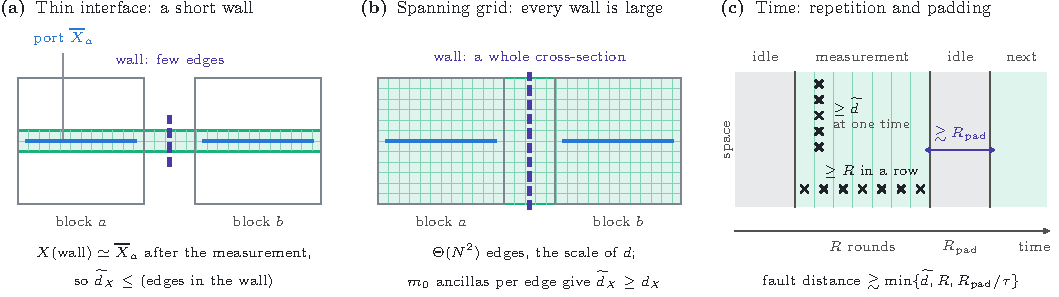
\includegraphics[width=\textwidth]{fault_distance_intuition.pdf}
\caption{Why the measurement keeps the fault distance, in a side view of two
blocks (squares) with their $X$ slab ports (blue) and the ancilla grid (green).
(a) If the grid joins the blocks only through a thin bridge, $X$ on a wall
across the bridge (dashed) is equivalent to $\overline X_a$ once
$\overline X_a\overline X_b$ is measured, so a few faults cause a logical error.
(b) If the grid fills both blocks, every wall between their ports is a whole
cross-section, with $\Theta(N^2)$ edges, the same scale as the code distance;
$m_0$ ancillas per edge make every wall at least as heavy as the ports it
separates, and the full distance is kept.  (c) In time, an undetected error
inside a measurement is either a logical at one time step, with at least
$\widetilde d$ faults, or one outcome wrong in each of the $R$ repeated rounds.
Idle rounds between operations force any pattern that links two of them to
stretch across the padding.}
\label{fig:fault-distance}
\end{figure*}

\textbf{Four ingredients keep the distance.}  First, the grid fills the
participating blocks, so every wall between their ports is a surface with
$\Omega(N^2)$ edges [Fig.~\ref{fig:fault-distance}(b)]; this is the constant
relative expansion of Eq.~\eqref{eq:grid-bound}, which the constant slab
thickness makes possible.  Second, carrying $m_0=\lceil2At\rceil$ parallel
ancillas on every grid edge multiplies every wall by $m_0$, so $\beta\ge1$ and
Eq.~\eqref{eq:gauge-distance} gives $\widetilde d_X\ge d_X$: each measurement
keeps the full static distance at constant ancilla cost.  Third, the
measurement is repeated in time [Fig.~\ref{fig:fault-distance}(c)].  A single
wrong outcome of one vertex star flips the reported product, so the new checks
are measured for $R=\Theta(d)$ rounds, and a wrong outcome that is not repeated
is caught by comparing consecutive rounds.  Williamson and Yoder proved the
resulting bound for gauging \cite{WilliamsonYoderGauging}; because our
operations start and end in open idle rounds rather than at perfect boundaries,
we give a direct proof.  Faults of the measured type ($X$) leave an error on the
data and a set of flipped edge readouts that together form an operator of the
deformed code, which is a nontrivial logical whenever they cause an error, so
there are at least $\widetilde d_X$ of them.  Faults of the other type either
leave a logical error on the data, with at least $d_Z$ faults, or flip the
reported outcome; then either every one of the $R$ rounds contains a wrong
outcome, or a round without one shows that the errors so far form a logical
that anticommutes with the measured one, again with at least $d_Z$ faults.
Hence the measurement has fault distance at least
$\min\{\widetilde d_X,d_Z,R\}$, and exact minimization on small instances shows
that this bound is attained.  Fourth, successive measurements on a block are
separated by $\Theta(d)$ idle rounds, so faults that straddle two operations also
cost $\Omega(d)$ (Sec.~\ref{sec:ft}).

Resource transfer is the one place where blocks of different distance meet.
Joining a small block to a large one cannot expose the large block: the same
wall argument, applied to everything except the small block's own logical
qubits, shows that every other logical operator keeps the distance of the
larger block.  The small courier blocks below therefore carry only one
traveling resource each, and their errors are charged to distillation.  Every
logical qubit that is read later, other than a resource in transit, is
protected at every step by fault distance $\Omega(d)$.

\subsection{Gates and encoded resources}
\label{sec:gates}
Pure-$X/Z$ measurements suffice for the logical gate set.  A CNOT uses an
ancilla $a$ in $|+\rangle$ and the measurements
\begin{equation}
 Z_cZ_a\;(u),\qquad X_aX_t\;(v),\qquad Z_a\;(w),
 \label{eq:cnot}
\end{equation}
followed by the Pauli-frame update $Z_c^vX_t^{u\oplus w}$, where outcome bit
zero denotes eigenvalue $+1$.  For phase teleportation, prepare $a$ in
$R_\theta|+\rangle$ with $R_\theta=\operatorname{diag}(1,e^{i\theta})$, measure
$Z_dZ_a$ with bit $m$ and $X_d$ with bit $n$, and retain $a$.  The correction
\begin{equation}
 C_{mn}=R_{2\theta}^{m}Z_a^nX_a^m
 \label{eq:phase}
\end{equation}
produces $R_\theta|\psi\rangle$.  For $\theta=\pi/2$ this consumes
$|Y\rangle=S|+\rangle$; for $\theta=\pi/4$ it consumes $|A\rangle=T|+\rangle$,
with a possible $S$ correction using one additional $|Y\rangle$.  Exchanging $X$
and $Z$ gives $S_X=HSH$, and $SS_XS=e^{i\pi/4}H$.  These identities generate the
universal Clifford+$T$ set from one- and two-block measurements.

A physical resource enters at a designated bare port.  The raw qubit is
teleported into an encoded block by a joint $ZZ$ measurement and an $X$ readout;
all spectator logical classes keep distance $\Omega(d)$ in the quotient by the
resource's weight-one error class.  Subsequent transfers use only encoded
blocks, with distances growing by fixed factors; we call this sequence an
encoded courier.  The resource supply uses fixed Steane $7\!\to\!1$ and
punctured Reed--Muller $15\!\to\!1$ factories built from the same logical
primitives \cite{BravyiKitaev,Reichardt,LitinskiMSD}.  Resource errors are
modeled as local-stochastic defective slots: a defective candidate may be in any
state, entangled with other candidates or with the environment.  Phase
teleportation with any such resource applies, relative to the ideal rotation, an
operator in $\operatorname{span}\{I,Z\}$ on the coordinate it feeds, so a
predetermined recovery returns exactly the ideal output whenever at most one
coordinate of a run is defective.  Each run therefore always produces an output,
and the outputs are again a defective family with
\begin{equation}
 q_{r+1}\le C_{\rm dist}q_r^2,\qquad C_{\rm dist}=\tbinom{30}{2}=435,
 \label{eq:distill}
\end{equation}
counting pairs among the fifteen principal and fifteen correction slots of a
run.  No twirl or diagonal error basis is assumed, and the raw boundary, encoded
transfers and factories are included in the circuit analysis rather than
supplied as ideal resources.

\subsection{Fault tolerance of the complete circuit}
\label{sec:ft}
The argument that the whole computation keeps fault distance $\Omega(d)$ has a
simple shape.  An undetected logical error needs a fault pattern that no
detector notices.  Split such a pattern into connected pieces, where two faults
are connected when they can trigger a common detector; at least one piece causes
the error.  A piece inside one operation and the idle rounds around it needs at
least $\min\{d,R\}$ faults, by Sec.~\ref{sec:distance}.  Successive operations
on a block are separated by $R_{\rm pad}$ idle rounds, and two connected faults
are at most $\tau=O(1)$ rounds apart, so a piece that reaches from one operation
to the next must stretch across the padding.  Precisely, with
$\delta_g^{\rm rel}$ the fault distance of measurement window $g$ and
$\delta_{\rm mem}^{\rm rel}$ that of idle memory, the composed phenomenological
distance satisfies
\begin{equation}
 f_{\rm ph}\ge\min\left\{
 \min_g\delta_g^{\rm rel},\delta_{\rm mem}^{\rm rel},
 1+\left\lfloor\frac{R_{\rm pad}-\tau}{\tau}\right\rfloor
 \right\},
 \label{eq:composition}
\end{equation}
with $\delta_g^{\rm rel}\ge\min\{\beta_0d,R_g\}$ for a window of $R_g$ rounds and
$\delta_{\rm mem}^{\rm rel}\ge d$.  Choosing $R_g$ and $R_{\rm pad}$ of order $d$
makes every term $\Omega(d)$.

The technical work lies in making ``inside one operation'' precise without
assuming that each operation starts from a perfect state.  We cut the schedule
in time at idle rounds and carry three pieces of data across each cut: the
syndrome $s$ left by earlier errors, the logical Pauli correction $\lambda$
accumulated so far, and the outcomes $\rho$ of the last measurement round, which
the next detectors compare against.  The records must be carried separately,
because a wrong outcome in the last round before a cut changes $\rho$ but not the
state.  With these three variables adjacent operations compose exactly; a direct
simulation of an idle$\,\to\,$gauging$\,\to\,$idle$\,\to\,$gauging$\,\to\,$idle
schedule on explicit layer-code blocks agrees with the composed map on every
single fault, and gluing without $\rho$ fails.  Each piece of a fault pattern is
then judged by its effect relative to the same schedule without it, which
removes every dependence on earlier errors.

Resource errors need one more step, because the courier blocks have smaller
distance.  A new error first created at courier stage $j$ needs a connected fault
pattern of size $\Omega(d_j)$; the raw injection stage is charged separately,
with a constant.  Distinct resources are kept far apart in spacetime, so one
short connected pattern cannot corrupt two of them: a chain of connected faults
can leave the courier blocks of one resource only through its transfer into the
factory block, and from there it must cross the $R$ idle rounds that separate
the transfer from every other operation on that block.  A script builds a
complete factory schedule by these rules, with cell reuse and adaptive branches,
and checks this separation on it.  Summing over the stages gives a resource
error $q_0=O(\sqrt p)$, which Eq.~\eqref{eq:distill} then suppresses
quadratically.

Every detector has bounded support, so the graph that connects faults through
common detectors has bounded degree.  The committed decoder chooses a
minimum-cardinality fault set consistent with the detector history through a
fixed buffer beyond the commitment time.  A wrong decision about a protected
outcome requires a large connected set of fault locations, a fixed fraction of
which are actual faults, and counting such sets in a bounded-degree graph yields
a positive threshold.  This decoder is information-theoretic; efficient
classical decoding is not assumed.

\subsection{Architecture theorem and resource scaling}
\label{sec:architecture}
The input family is a balanced good CSS LDPC family with boundedly dense sizes:
every sufficiently large target length has an available member within a fixed
factor.  Fixed-degree quantum Tanner codes provide such a family
\cite{LeverrierZemorTanner,DinurLTC}.  Let $A\subset\mathbb Z^3$ be the logical
region, $W=|A|$, and $T$ the logical circuit depth.  Partition the logical
lattice into boxes of side $b(f)=\Theta(f^{1/6})$, and let $B_f(A)$ count the
boxes that meet $A$ but are not completely filled.

\begin{theorem}[Universal fault-tolerant architecture]
\label{thm:architecture}
Use the explicit realization of Theorem~\ref{thm:slabs}, a balanced good input
family with boundedly dense sizes, and the local measurement, resource and
extraction schedules above.  There are constants $p_{\rm th},c,f_{\min}>0$ such
that for $0<p<p_{\rm th}$ and target failure $0<\varepsilon<1/2$, any finite
nearest-neighbor three-dimensional logical circuit can be simulated with
\begin{equation}
 f=\max\left\{f_{\min},
 \left\lceil\frac{c\log(WT/\varepsilon)}{\log(p_{\rm th}/p)}\right\rceil
 \right\},
 \label{eq:f}
\end{equation}
using
\begin{align}
 Q_{\rm phys}&=O\!\left(Wf+(B_f(A)+1)f^{3/2}\right),
 \label{eq:space}\\
 D_{\rm phys}&=O(Tf^{3/2}\Psi),\qquad \Psi=O(f^{\log_215}).
 \label{eq:depth}
\end{align}
Persistent data remain in layer-code blocks, and physical operations use
nearest-neighbor connectivity.  For a connected bounded-aspect logical box,
$Q_{\rm phys}=O(Wf+f^{3/2})$.
\end{theorem}

The scaling follows directly from the code parameters.  Choose $d=\Theta(f)$
and measurement, padding and commitment buffers of order $f$.
Equation~\eqref{eq:parameters} then gives $N=\Theta(\sqrt f)$,
$K=\Theta(\sqrt f)$ and $n=\Theta(f^{3/2})$ per cell.  A full coarse box fits
into one cell, so $O(W/K+B_f(A)+1)$ cells suffice, and multiplication by $n$
proves Eq.~\eqref{eq:space}; for a bounded-aspect box
$B_f(A)=O((W/\sqrt f)^{2/3}+1)$ is absorbed (Fig.~\ref{fig:resources}).  For
time, a distilled resource takes $O(f\Psi)$ rounds, where $\ell$ distillation
levels give $\Psi=O(15^\ell)$ and $2^\ell=O(f)$.  One logical layer needs $O(K)$
resources per data block, and serial production gives
$O(Kf\Psi)=O(f^{3/2+\log_215})\subseteq O(f^{5.41})$ rounds per layer, against
$O(f)$ for lattice surgery.  The serial schedule minimizes space, not space-time
volume: with $P$ factories per cell the space becomes $O(WfP+f^{3/2})$ and the
depth $O(TKf\Psi/P)$.

\begin{figure*}[t]
\centering
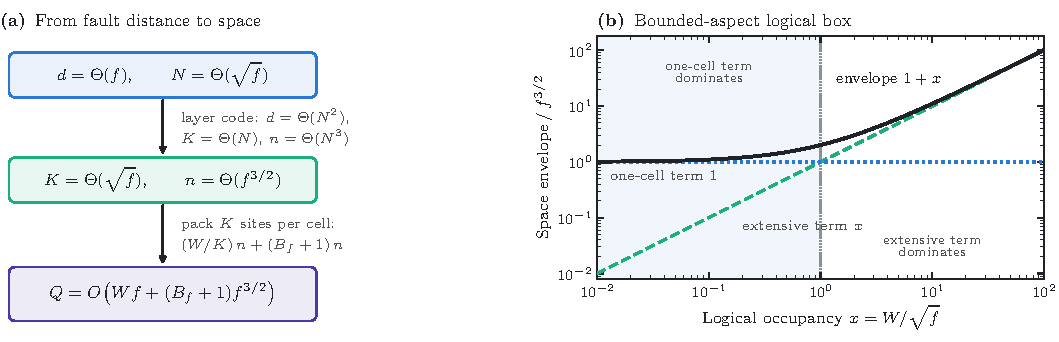
\includegraphics[width=\textwidth]{revision_resources.pdf}
\caption{Origin and crossover of the resource bound. (a) Target fault distance
$f$ fixes the cell parameters; packing $K=\Theta(\sqrt f)$ logical sites per
cell yields an extensive $Wf$ term plus the cost of partially occupied cells.
(b) For bounded-aspect boxes, the normalized scaling envelope is proportional to
$1+x$, where $x=W/\sqrt f$.  The one-cell term dominates for $x\ll1$ and the
extensive term for $x\gg1$.  Constants are suppressed: this illustrates the
asymptotic bound and is not a numerical qubit estimate.}
\label{fig:resources}
\end{figure*}

\textbf{Concrete estimate.}  An estimate with stated constants, explicit integer
allocations and distances chosen from each schedule's complete runtime makes the
scales explicit.  For $W=100$ sites, $T=10^6$ layers, $\varepsilon=10^{-2}$,
$p=10^{-3}$ and injected resource error $10^{-2}$, the always-output
distillation covered by the theorem does not converge: Eq.~\eqref{eq:distill}
requires an injected error below $1/C_{\rm dist}\approx2.3\times10^{-3}$.  With
optimistic postselected distillation, which the theorem does not cover, the
serial layer-code schedule needs about $10^9$ qubits for two months, against
$4\times10^5$ qubits for three days for a serial surface-code layout and
$2\times10^8$ qubits for $23$\,s for a throughput-limited one.  At these
distances a layer-code block holds one to three logical qubits; with the same
accounting on both sides it stores a logical qubit more cheaply than a
surface-code patch only for $d\gtrsim1100$ (between about $600$ and $2300$
across scenarios).  The asymptotic advantage is therefore far from the
practical regime until these constants, and the distillation protocol, improve.

\subsection{Port packing and shallow logical gates}
\label{sec:structure}
Slab mobility also constrains how logical information can be spatially
accessible.  For a region $A$, let $g_X(A)$ be the dimension of the pure-$X$
logical space supported in $A$, and define $g_Z(B)$ analogously.  The rank
$r(A,B)$ of their commutation pairing obeys
\begin{equation}
 \max\{0,g_X(A)+g_Z(B)-K\}\le r(A,B)\le |A\cap B|,
 \label{eq:overlap}
\end{equation}
because all cross commutation factors through the intersection and the full
logical pairing is nondegenerate.  If $A_1,\ldots,A_{r_X}$ are disjoint complete
$X$ ports and $B_1,\ldots,B_{r_Z}$ disjoint complete $Z$ ports, summing over all
pairs gives the crossbar bound
\begin{equation}
 r_Xr_ZK\le n.
 \label{eq:crossbar}
\end{equation}
For the balanced layer-code slabs $r_X,r_Z=\Theta(N)$, $K=\Theta(N)$ and
$n=\Theta(N^3)$, so the bound is saturated: the cubic size is optimal among CSS
families required to provide $\Theta(K)$ disjoint complete ports in both
polarizations.  Pairing the $i$th $X$-slab and $Z$-slab representatives of any
logical Pauli also gives disjointness $\Delta=\Theta(N)$, with smallest and
largest logical weights $\Theta(N^2)$.  The Jochym-O'Connor--Kubica--Yoder
criterion \cite{JochymDisjointness} then forces every fixed-depth,
bounded-arity, code-preserving unitary on a large static block to be logical
Clifford.  This is why the architecture uses adaptive measurements and resource
states, which lie outside that unitary setting.

\subsection{Simulations on explicit layer-code blocks}
\label{sec:sim-results}
\begin{figure*}[t]
\centering
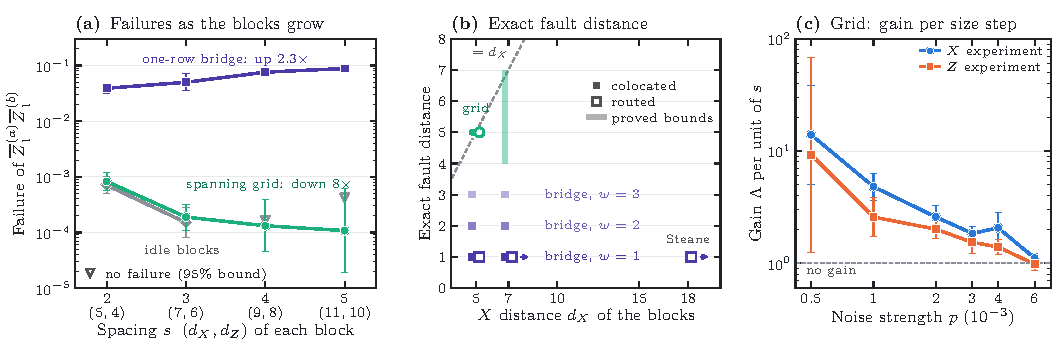
\includegraphics[width=\textwidth]{two_block_main.pdf}
\caption{Two-block logical measurement on explicit layer-code blocks: the cut
obstruction at scale, in simulation (the hardware counterpart is
Fig.~\ref{fig:hardware}).  (a)~Failure of the measured pair
$\overline Z_1^{(a)}\overline Z_1^{(b)}$ at $p=10^{-3}$ as the block spacing $s$
grows, through a one-row bridge (violet), a spanning grid (aqua), and for the
blocks left idle (grey), with Wilson 95\% intervals (open triangles: upper ends
of zero counts).  (b)~Exact circuit fault distance against the $X$ distance of
the blocks, computed by CP-SAT.  Filled: colocated ancillas at $s=2,3$; open:
routed nearest-neighbor extraction at $s=2$ with the $[[4,2,2]]$, band and
Steane inputs (block $X$ distances $5$, at least $7$ and at least $18$, arrows);
bar: proved lower bound and the weight of an undetectable pattern where the
solver stopped.  Through a bridge of $w$ rows the distance stays at $w$; through
the grid it equals $d_X$ (dashed) where resolved.  (c)~Factor $\Lambda$ by which
each unit of spacing suppresses failures through the spanning grid, with 95\%
intervals.}
\label{fig:two-block}
\end{figure*}

\textbf{Exact fault distances.}  Without noise every detector and all eight
observables are deterministic, so the circuit implements the projective
measurement with the correct outcome and leaves the spectators untouched.  On
two $[[4,2,2]]$ blocks at $s=2$ ($n=224$, distances $5$ and $4$), the fault
distance of $\overline Z_1^{(a)}\overline Z_1^{(b)}$ through a bridge of $w=1,2,3$
rows is exactly $w$; for $w=1$ a single fault suffices
[Fig.~\ref{fig:two-block}(b)].  This is the cut obstruction at circuit level.  A
grid spanning both blocks restores it to exactly $5$, the blocks' $X$ distance,
while the fault distances of the reported bit, set by the number of rounds, and
of the spectators do not depend on the interface.  At $s=3$ the bridge distance
is still exactly $w$, although the blocks' $X$ distance is now $7$.

\textbf{Failure rates.}  At $p=10^{-3}$ the failure rate of
$\overline Z_1^{(a)}\overline Z_1^{(b)}$ through the one-row bridge rises from
$3.9\%$ at $s=2$ to $8.8\%$ at $s=5$, because the undetectable bridge fault has
more rounds in which to occur, while through the spanning grid it falls from
$8.2\times10^{-4}$ to about $10^{-4}$ and agrees with the same blocks left idle
[Fig.~\ref{fig:two-block}(a)].  For the spanning grid each unit of spacing
suppresses failures by a factor $\Lambda=4.8$ in the $X$ experiment and $2.6$ in
the $Z$ experiment at $p=10^{-3}$, falling to one near $p\approx6\times10^{-3}$
[Fig.~\ref{fig:two-block}(c)].

\textbf{Routed circuits.}  Without noise all $28$ routed measurement circuits
implement the measurement exactly, and the $12$ idle controls also give silent
detectors and correct observables.  Through the one-row bridge the fault
distance is exactly $1$ for all three inputs, although the blocks' $X$ distance
grows from $5$ to at least $18$.  On the $[[4,2,2]]$ blocks with $R=5$ the
spanning grid gives exactly $5$, the same as the blocks left idle; the reported
bit has exactly $5=R$, and the spectator frames exactly $4=d_Z$, as in idle
memory, so routing leaves the distances of the colocated circuit unchanged where
both are resolved.  On the band blocks the reported bit has an undetectable
pattern of weight $6$ at $R=7$, which the block itself explains: its lightest
$Z$-type operator that anticommutes with the measured logical has weight $6$.  At
the tested noise strengths the sampled failure rates of these long routed
circuits do not distinguish the interfaces, so we use only their exact
distances.

\textbf{Surface-code campaign.}  All 15 noiseless controls have zero failures.
For every gauged duration the failure rate decreases monotonically with $L$
across all five sizes at every tested $p\le0.004$.  At $p=0.0035$ increasing $L$
from 3 to 11 reduces the failure rate from $0.1111$ to $0.0324$ for $G=d$, and
at $p=0.0015$ (also $G=d$) the reduction is about $6.5\times10^2$.  Tripling the gauged
duration shifts the smallest-versus-largest crossing by about $3.2\%$, from
$4.47\times10^{-3}$ to $4.33\times10^{-3}$.  These are finite-size diagnostics of
a surface-code model, not estimates of the theorem's threshold.

\subsection{Hardware demonstrations}
\label{sec:hw-results}
Figure~\ref{fig:hardware} shows what was run and what was measured, and
Table~\ref{tab:hardware} collects the tests.  Each of the three predicted gains
appears on hardware; the exceptions are noted below.

\begin{figure*}[t]
\centering
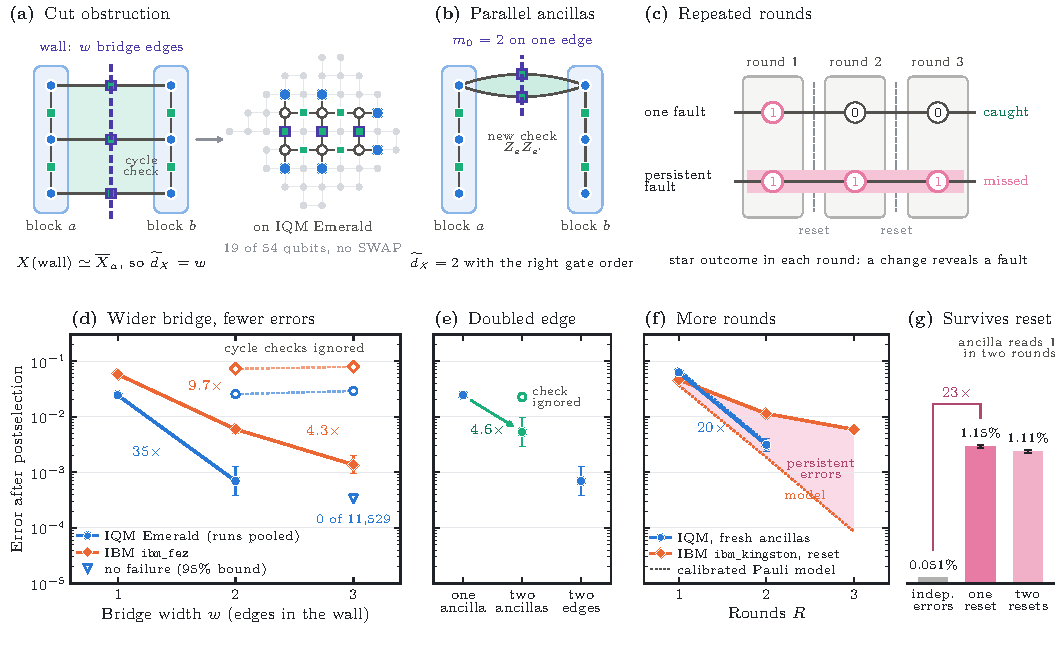
\includegraphics[width=\textwidth]{hardware_overview.pdf}
\caption{Hardware demonstrations of the three distance mechanisms.  Top row:
what was run.  (a)~Two three-qubit blocks (blue) joined by a bridge of $w$ edges,
each with an edge ancilla (aqua squares); $X$ on the wall of bridge edges
(violet) is equivalent to $\overline X_a$, so the deformed $X$ distance and the
exact circuit fault distance are both $w$.  Shaded: the cycle checks that the
extra bridge edges create.  Right: the circuit for $w=3$ as placed on IQM
Emerald, with the couplers it uses.  (b)~Two parallel ancillas on one bridge
edge ($m_0=2$) add the two-edge check $Z_eZ_{e'}$.  (c)~A wrong star outcome in
one round is revealed by the change in the next round; a fault that persists
across rounds repeats the same wrong outcome and is missed.  Bottom row: what
was measured, as the error after postselection on every detector, with Wilson
95\% intervals (open triangle: upper end of a zero count).  (d)~IQM runs pooled;
open symbols: the same samples with the cycle checks ignored.  (e)~IQM, one
bridge edge with one or two ancillas, and two bridge edges; open symbol: the
two-edge check ignored.  (f)~Reported-bit error against the number of rounds
$R$, with the calibrated Pauli models (dotted); IQM uses fresh ancillas in every
round, \texttt{ibm\_kingston} measures and resets them.  Shaded: the excess over
the model (run A).  (g)~Rate at which a check ancilla on \texttt{ibm\_kingston}
(run B) reads 1 in two consecutive rounds with no data error to explain it,
against the rate that independent errors give, with one or two resets between
rounds.}
\label{fig:hardware}
\end{figure*}

\begin{table*}[t]
\centering
\caption{Hardware tests.  Error after postselection on every detector;
one-sided Fisher exact tests.  P: test fixed before the run.  Control: the same
samples with the checks of the better interface ignored.}
\label{tab:hardware}
\small
\begin{tabular}{@{}lllcl@{}}
\toprule
Device & Comparison & Error & Gain & $p$ value\\
\midrule
\multicolumn{5}{@{}l}{\emph{Cut obstruction}}\\
IQM Emerald & $w=1\to2$ & $\hwIQMwOne\%\to\hwIQMwTwo\%$ & \hwIQMfold$\times$ & $\le\hwIQMpOneTwo$ (each run)\\
 & $w=2\to3$ & $\hwIQMwTwo\%\to0$ of \hwIQMwThreeKept & & \hwIQMpTwoThree{} (P, not met)\\
 & control, $w=2,3$ & \hwIQMctrl\% & & \\
IBM \texttt{ibm\_fez} & $w=1\to2$ & $\hwIBMwOne\%\to\hwIBMwTwo\%$ & \hwIBMfoldOneTwo$\times$ & \hwIBMpOneTwo\\
 & $w=2\to3$ & $\hwIBMwTwo\%\to\hwIBMwThree\%$ & \hwIBMfoldTwoThree$\times$ & \hwIBMpTwoThree\\
 & control, $w=2,3$ & \hwIBMctrl\% & & \\
\multicolumn{5}{@{}l}{\emph{Parallel ancillas}}\\
IQM Emerald & one $\to$ two ancillas & $\hwIQMwOne\%\to\hwMult\%$ & \hwMultFold$\times$ & \hwMultP\\
 & control & \hwMultCtrl\% & & \\
\multicolumn{5}{@{}l}{\emph{Repeated rounds}}\\
IQM Emerald & $R=1\to2$, fresh ancillas & $\hwRndIQMOne\%\to\hwRndIQMTwo\%$ & \hwRndIQMfold$\times$ & \hwRndIQMp{} (P)\\
 & model & $\hwRndIQMModelOne\%\to\hwRndIQMModelTwo\%$ & & \\
IBM \texttt{ibm\_kingston} & $R=1\to2\to3$, reset & $\hwRndIBMOne\%\to\hwRndIBMTwo\%\to\hwRndIBMThree\%$ & & \hwRndIBMpOneTwo{} (P)\\
 & model, $R=2,3$ & \hwRndIBMModelTwo\%, \hwRndIBMModelThree\% & & \\
\multicolumn{5}{@{}l}{\emph{Ancilla errors that survive a reset}}\\
IBM \texttt{ibm\_kingston} & one $\to$ two resets & $\hwPersSingle\%\to\hwPersDouble\%$ & & \hwPersP{} (P)\\
 & independent errors & \hwPersIndep\% & & \\
\bottomrule
\end{tabular}
\end{table*}

\textbf{Cut obstruction.}  The postselected error falls \hwIQMfold-fold, from
\hwIQMwOne\% at $w=1$ to \hwIQMwTwo\% at $w=2$, on IQM (pooled over three runs on
two sets of qubits; $p\le\hwIQMpOneTwo$ in each of the two runs with both
widths), and on IBM from \hwIBMwOne\% to \hwIBMwTwo\% and \hwIBMwThree\% at
$w=1,2,3$, by factors of \hwIBMfoldOneTwo{} and \hwIBMfoldTwoThree{}
[Fig.~\ref{fig:hardware}(a,d)].  When the cycle checks that the extra bridge
edges create are ignored, the error returns to the width-one level (\hwIQMctrl\%
on IQM, \hwIBMctrl\% on IBM), so the gain comes from the larger wall and not from
discarding more samples.  On IQM width three had no failure in
\hwIQMwThreeKept{} kept samples, but its difference from width two is not
significant ($p=\hwIQMpTwoThree$, in a test fixed before the run): width two was
already too rare to resolve.  The IBM errors exceed the model, which assumed
typical published error rates and no idle or crosstalk errors.

\textbf{Parallel ancillas.}  Two parallel ancillas on a single bridge edge
($m_0=2$) give \hwMult\% instead of \hwIQMwOne\%, a \hwMultFold-fold gain
($p=\hwMultP$), and \hwMultCtrl\% when the new two-edge check is ignored
[Fig.~\ref{fig:hardware}(b,e)].  The first CNOT order we tried had circuit fault
distance one: a fault on the vertex ancilla between its two bridge CNOTs put $X$
on both parallel edges, which the two-edge check cannot see.  Separating the two
CNOTs restores distance two.  This is the constant-factor loss from circuit
faults that Sec.~\ref{sec:noise} allows for; a suitable CNOT order avoids it.

\textbf{Repeated rounds and errors that survive a reset.}  With fresh ancillas
in each round (IQM) the reported-bit error falls \hwRndIQMfold-fold, from
\hwRndIQMOne\% at $R=1$ to \hwRndIQMTwo\% at $R=2$, close to the model's
\hwRndIQMModelOne\% and \hwRndIQMModelTwo\% ($p=\hwRndIQMp$, fixed in advance).
On IBM, where the ancillas are measured and reset between rounds, it falls from
\hwRndIBMOne\% to \hwRndIBMTwo\% and \hwRndIBMThree\% for $R=1,2,3$ (both steps
$p\hwRndIBMpOneTwo$, fixed in advance), but far less than the calibrated model
predicts (\hwRndIBMModelTwo\% and \hwRndIBMModelThree\% at $R=2,3$); at $R=3$
the error is \hwRndIBMModelRatio~times the prediction
[Fig.~\ref{fig:hardware}(f)].  The cause is an ancilla error that survives the
reset: a check ancilla reads 1 in two consecutive rounds, with no data error to
explain it, in \hwPersSingle\% of samples, \hwPersRatio~times the rate that
independent errors give, and a second reset removes only \hwPersRel\% of these
events ($p=\hwPersP$) [Fig.~\ref{fig:hardware}(g)].  Such a fault, most likely
leakage out of the qubit subspace, corrupts the same outcome in every round.  It
lies outside the local-stochastic model of Sec.~\ref{sec:noise}, which charges
every round separately.

%======================================================================
\section{Discussion}
\label{sec:discussion}
%======================================================================
\textbf{What the results mean.}  The answer to the research question is yes,
under the stated noise model.  Prefix-parity repair exposes logical operators in
single-layer slabs of an explicit realization; grid gauging turns those slabs
into protected measurements; and a composed detector schedule supports resource
transfer and distillation in the same geometry.  Because a layer-code distance
is comparable to the area of a block face, every joint measurement must cross a
constant fraction of that face.  A thick grid does so and, with a constant
ancilla multiplicity, keeps the full distance, whereas a thin measurement layer
cannot.  The simulations on layer-code blocks (Fig.~\ref{fig:two-block}) and the
hardware runs (Fig.~\ref{fig:hardware}) show this contrast.  The hardware runs
reproduce at small scale the three facts that the distance argument combines:
the smallest wall bounds the distance of a joint measurement, parallel ancillas
widen every wall that crosses their edge, and repeated rounds protect the
reported bit.  For bounded-aspect logical regions the space bound separates an
extensive $Wf$ cost from the minimum $f^{3/2}$ cost of one encoded cell, and the
port-packing result gives a second reading of the layer-code parameters: their
cubic volume supports linearly many disjoint complete ports of each
polarization.

\textbf{Limitations.}  (i) The threshold is existential, and the decoder is
minimum-weight, which is not efficient; a practical decoder for deformation
histories is open.  (ii) The constants are large: the storage advantage over
surface codes appears only near $d\approx1100$, and the distillation covered by
the theorem needs injected errors below $2.3\times10^{-3}$.  (iii) The
fault-distance bounds are proved in the phenomenological model and transferred
to circuits through the constant $c_1$; exact minimization checks them only on
small instances.  (iv) The hardware blocks
are three-qubit codes, so the runs do not test layer codes, the grid expansion,
the threshold or the resource scaling, which need far larger devices.  The
\texttt{ibm\_fez} circuits were routed rather than SWAP-free, the first runs'
tests were chosen after the data, and the pre-registered IQM test of width two
against three was not met.  (v) Ancilla errors that persist across rounds, most
likely leakage, violate the local-stochastic assumption, so any implementation
of the extraction schedule would need leakage reduction.

\textbf{Future work.}  The next steps are a practical decoder for deformation
histories, with changing checks, inherited frames and records, and joint
measurements (the layer-code decoders of Ref.~\cite{GuRandomLayerCodes2026} are a
natural starting point); routed circuit-level benchmarks on inputs that grow into
the balanced regime; bounds on how many logical measurements can share the slab
interfaces, compared with parallel code surgery \cite{CowtanParallelSurgery};
factories with smaller constants; and an extension of the fault-path analysis to
leakage and coherent noise.  Random layer codes built from random CSS inputs
\cite{GuRandomLayerCodes2026} are a natural candidate for reducing the
constants; the explicit realization applies to any CSS input, but the resource
accounting would need their parameter scaling.

%======================================================================
\section{Conclusion}
\label{sec:conclusion}
%======================================================================
Three-dimensional layer codes can do more than store quantum information.  Every
pure logical operator of an explicit layer-code lattice has a representative in
a single movable layer, and a local three-dimensional ancilla grid measures it
without losing the optimal distance $\Theta(N^2)$, while every thin measurement
interface provably fails.  Built into a universal fault-tolerant architecture,
these measurements keep the optimal storage cost, $O(Wf+f^{3/2})$ physical qubits
for $W$ logical sites.  Simulations on explicit layer-code blocks and experiments
on IQM and IBM processors confirm the distance mechanisms, and the experiments
identify ancilla errors that survive a reset as the main assumption that present
hardware does not meet.

%======================================================================
\section*{Data and code availability}
\addcontentsline{toc}{section}{Data and code availability}
%======================================================================
All code and data are in the public project repository \cite{Repo}:
\begin{center}
\href{\repourl}{\texttt{\small github.com/HellWithCode0/}}\\
\href{\repourl}{\texttt{\small layer-code-fault-tolerance}}
\end{center}
It contains:
\begin{itemize}\raggedright
\item \texttt{iris\_paper/}: this paper, its source and figures;
\item \texttt{supplement.pdf}: a technical report with the complete proofs, and
\texttt{manuscript.pdf}, the companion journal manuscript;
\item \texttt{layer\_code\_explicit.py} and \texttt{slab\_gluing\_certificate.py}:
the explicit lattice, its check matrices and the slab certificates;
\item \texttt{two\_block\_measurement.py}, \texttt{scaling\_campaign/} and
\texttt{numerical/}: the simulations, circuits, and every batch of samples with
its seed;
\item \texttt{min\_weight\_logical.py}: exact fault distances with CP-SAT;
\item \texttt{hardware/}: the hardware circuits, job identifiers, raw outputs,
calibration snapshots and analysis scripts;
\texttt{hardware/hardware\_summary.py} computes the hardware numbers of
Sec.~\ref{sec:hw-results} and Table~\ref{tab:hardware} from the raw outputs;
\item \texttt{make\_*\_figure.py}: the figure scripts.
\end{itemize}
The repository README lists how to rerun each check.

%======================================================================
\section*{Acknowledgements}
\addcontentsline{toc}{section}{Acknowledgements}
%======================================================================
The author thanks Dominic J. Williamson for helpful correspondence.  Williamson
pointed out that adding logical-measurement layers to a layer code can, in
principle, reduce its fault distance, noted that this question had been left open
in an earlier idea of performing universal computation on layer codes by adding
such layers, and suggested that random layer codes \cite{GuRandomLayerCodes2026}
may be useful here.  Section~\ref{sec:distance} and the corresponding results of
the technical report (the cut obstruction, the edge-multiplicity result, the
encoded-port quotient, and the distance ledger) were added in response.  He later
suggested that the junction construction and the fault-distance argument be
explained in plainer terms, and those parts were rewritten for that purpose.  The
correspondence did not include a detailed review of the proofs, and any errors
are the author's own.  The IQM experiments used the Open Quantum platform
\cite{OpenQuantum2026}.  We acknowledge the use of IBM Quantum services for this
work.  The views expressed are those of the author, and do not reflect the
official policy or position of IBM or the IBM Quantum team.

\section*{Acknowledgment of AI assistance}
\addcontentsline{toc}{section}{Acknowledgment of AI assistance}
Claude Code assisted with manuscript organization, language editing, figure
preparation, and scripts from the supplied research materials and numerical
data.

%======================================================================
\renewcommand{\refname}{References}
\addcontentsline{toc}{section}{References}
{\small
\setlength{\itemsep}{0pt}
\begin{thebibliography}{99}
\bibitem{BPT}
S. Bravyi, D. Poulin, and B. Terhal, Tradeoffs for reliable quantum information storage in 2D systems, Phys. Rev. Lett. \textbf{104}, 050503 (2010), \href{https://arxiv.org/abs/0909.5200}{arXiv:0909.5200}.

\bibitem{HorsmanLatticeSurgery}
D. Horsman, A. G. Fowler, S. Devitt, and R. Van Meter, Surface code quantum computing by lattice surgery, New J. Phys. \textbf{14}, 123011 (2012), \href{https://arxiv.org/abs/1111.4022}{arXiv:1111.4022}.

\bibitem{LitinskiSurgery}
D. Litinski, A game of surface codes: large-scale quantum computing with lattice surgery, Quantum \textbf{3}, 128 (2019), \href{https://arxiv.org/abs/1808.02892}{arXiv:1808.02892}.

\bibitem{VasmerBrowne}
M. Vasmer and D. E. Browne, Three-dimensional surface codes: Transversal gates and fault-tolerant architectures, Phys. Rev. A \textbf{100}, 012312 (2019), \href{https://arxiv.org/abs/1801.04255}{arXiv:1801.04255}.

\bibitem{WilliamsonBaspinLayerCodes}
D. J. Williamson and N. Baspin, Layer codes, Nat. Commun. \textbf{15}, 9528 (2024), \href{https://arxiv.org/abs/2309.16503}{arXiv:2309.16503}.

\bibitem{WilliamsonYoderGauging}
D. J. Williamson and T. J. Yoder, Low-overhead fault-tolerant quantum computation by gauging logical operators, Nat. Phys. \textbf{22}, 598 (2026), \href{https://arxiv.org/abs/2410.02213}{arXiv:2410.02213}.

\bibitem{CowtanParallelSurgery}
A. Cowtan, Z. He, D. J. Williamson, and T. J. Yoder, Parallel logical measurements via quantum code surgery, PRX Quantum \textbf{7}, 020325 (2026), \href{https://doi.org/10.1103/gj8x-n5gg}{doi:10.1103/gj8x-n5gg}.

\bibitem{IdeHomological}
B. Ide, M. G. Gowda, P. J. Nadkarni, and G. Dauphinais, Fault-tolerant logical measurements via homological measurement, Phys. Rev. X \textbf{15}, 021088 (2025), \href{https://doi.org/10.1103/PhysRevX.15.021088}{doi:10.1103/PhysRevX.15.021088}.

\bibitem{YuanParsimonious2026}
A. C. Yuan, A. Cowtan, Z. He, T.-C. Lin, and D. J. Williamson, Parsimonious quantum low-density parity-check code surgery, \href{https://arxiv.org/abs/2603.05082}{arXiv:2603.05082} (2026).

\bibitem{BerentLiftedSurgery}
L. Berent, L. Z. Cohen, and A. O. Quintavalle, Lifted surgery: Fast processing with QLDPC codes, \href{https://arxiv.org/abs/2609.11723}{arXiv:2609.11723} (2026).

\bibitem{SwaroopAdapters}
E. Swaroop, T. Jochym-O'Connor, and T. J. Yoder, Universal adapters between quantum low-density parity-check codes, PRX Quantum \textbf{7}, 010324 (2026), \href{https://arxiv.org/abs/2410.03628}{arXiv:2410.03628}.

\bibitem{HeExtractors}
Z. He, A. Cowtan, D. J. Williamson, and T. J. Yoder, Extractors: qLDPC architectures for efficient Pauli-based computation, \href{https://arxiv.org/abs/2503.10390}{arXiv:2503.10390} (2025).

\bibitem{ZhangGoodQLDPC}
G. Zhang, Y. Zhu, and Y. Li, Accelerating fault-tolerant quantum computation with good quantum low-density parity-check codes, PRX Quantum \textbf{7}, 033012 (2026), \href{https://doi.org/10.1103/3fj5-gn1h}{doi:10.1103/3fj5-gn1h}.

\bibitem{MalcolmEfficientQLDPC}
A. J. Malcolm, A. N. Glaudell, P. Fuentes, \emph{et al.}, Computing efficiently in QLDPC codes, Nat. Commun. \textbf{17}, 7286 (2026), \href{https://doi.org/10.1038/s41467-026-73061-9}{doi:10.1038/s41467-026-73061-9}.

\bibitem{PattisonHierarchical}
C. A. Pattison, A. Krishna, and J. Preskill, Hierarchical memories: Simulating quantum LDPC codes with local gates, Quantum \textbf{9}, 1728 (2025), \href{https://arxiv.org/abs/2303.04798}{arXiv:2303.04798}.

\bibitem{ChoeKoenigLocal}
S. H. Choe and R. K\"onig, How to fault-tolerantly realize any quantum circuit with local operations, \href{https://arxiv.org/abs/2402.13863}{arXiv:2402.13863} (2024).

\bibitem{BaspinWire}
N. Baspin and D. J. Williamson, Wire codes, Quantum \textbf{10}, 2083 (2026), \href{https://arxiv.org/abs/2410.10194}{arXiv:2410.10194}.

\bibitem{YangPlanar}
Y. Yang, G. Zhang, and Y. Li, Planar fault-tolerant logical measurements with low qubit overhead, npj Quantum Inf. (2026), \href{https://doi.org/10.1038/s41534-026-01310-2}{doi:10.1038/s41534-026-01310-2}, \href{https://arxiv.org/abs/2506.18061}{arXiv:2506.18061}.

\bibitem{GottesmanFTThreshold}
D. Gottesman, Fault-tolerant quantum computation with constant overhead, Quantum Inf.\ Comput.\ \textbf{14}, 1338 (2014), \href{https://arxiv.org/abs/1310.2984}{arXiv:1310.2984}.

\bibitem{KovalevPryadko}
A.~A. Kovalev and L.~P. Pryadko, Fault tolerance of quantum low-density parity check codes with sublinear distance scaling, Phys.\ Rev.\ A \textbf{87}, 020304(R) (2013).

\bibitem{FawziGrospellierLeverrier}
O. Fawzi, A. Grospellier, and A. Leverrier, Constant overhead quantum fault tolerance with quantum expander codes, in \emph{FOCS 2018}, pp.\ 743--754 (2018), \href{https://arxiv.org/abs/1808.03821}{arXiv:1808.03821}.

\bibitem{ZhangInjectionIndependence}
G. Zhang, Y. Zhu, X. Yuan, and Y. Li, Constant-overhead magic state injection into qLDPC codes with error independence guarantees, \href{https://arxiv.org/abs/2505.06981}{arXiv:2505.06981} (2025).

\bibitem{LiuInSituInjection}
K. Liu, S. Xu, T. Jochym-O'Connor, Z. He, S. Singh, and Y. Ding, In-situ simultaneous magic state injection on arbitrary CSS qLDPC codes, \href{https://arxiv.org/abs/2604.05126}{arXiv:2604.05126} (2026).

\bibitem{Repo}
Project repository: code, data, hardware records and technical report for this paper, \url{https://github.com/HellWithCode0/layer-code-fault-tolerance} (2026).

\bibitem{Stim}
C. Gidney, Stim: a fast stabilizer circuit simulator, Quantum \textbf{5}, 497 (2021), \href{https://arxiv.org/abs/2103.02202}{arXiv:2103.02202}.

\bibitem{CPSAT}
L. Perron and F. Didier, CP-SAT solver, Google OR-Tools, \url{https://developers.google.com/optimization} (2024).

\bibitem{LSD}
T. Hillmann, L. Berent, A. O. Quintavalle, J. Eisert, R. Wille, and J. Roffe, Localized statistics decoding: A parallel decoding algorithm for quantum low-density parity-check codes, \href{https://arxiv.org/abs/2406.18655}{arXiv:2406.18655} (2024).

\bibitem{Wilson}
E. B. Wilson, Probable inference, the law of succession, and statistical inference, J. Am. Stat. Assoc. \textbf{22}, 209 (1927).

\bibitem{PyMatching}
O. Higgott and C. Gidney, Sparse Blossom: correcting a million errors per core second with minimum-weight matching, Quantum \textbf{9}, 1600 (2025), \href{https://arxiv.org/abs/2303.15933}{arXiv:2303.15933}.

\bibitem{OpenQuantum2026}
R. Kuhn, O. Armbruster, and B. Wold, Open Quantum: An open infrastructure layer for quantum computing, Zenodo preprint (2026), \href{https://doi.org/10.5281/zenodo.22103261}{doi:10.5281/zenodo.22103261}.

\bibitem{Qiskit}
A. Javadi-Abhari \emph{et al.}, Quantum computing with Qiskit, \href{https://arxiv.org/abs/2405.08810}{arXiv:2405.08810} (2024).

\bibitem{Fisher}
R. A. Fisher, On the interpretation of $\chi^2$ from contingency tables, and the calculation of P, J. R. Stat. Soc. \textbf{85}, 87 (1922).

\bibitem{BravyiKitaev}
S. Bravyi and A. Kitaev, Universal quantum computation with ideal Clifford gates and noisy ancillas, Phys. Rev. A \textbf{71}, 022316 (2005), \href{https://arxiv.org/abs/quant-ph/0403025}{arXiv:quant-ph/0403025}.

\bibitem{Reichardt}
B. W. Reichardt, Quantum universality from magic states distillation applied to CSS codes, Quantum Inf. Process. \textbf{4}, 251 (2005).

\bibitem{LitinskiMSD}
D. Litinski, Magic state distillation: not as costly as you think, Quantum \textbf{3}, 205 (2019).

\bibitem{LeverrierZemorTanner}
A. Leverrier and G. Z\'emor, Quantum Tanner codes, in \emph{2022 IEEE 63rd Annual Symposium on Foundations of Computer Science (FOCS)}, pp. 872--883 (2022), \href{https://doi.org/10.1109/FOCS54457.2022.00117}{doi:10.1109/FOCS54457.2022.00117}, \href{https://arxiv.org/abs/2202.13641}{arXiv:2202.13641}.

\bibitem{DinurLTC}
I. Dinur, S. Evra, R. Livne, A. Lubotzky, and S. Mozes, Locally testable codes with constant rate, distance, and locality, in \emph{Proceedings of the 54th Annual ACM SIGACT Symposium on Theory of Computing (STOC '22)}, pp. 357--374 (2022), \href{https://doi.org/10.1145/3519935.3520024}{doi:10.1145/3519935.3520024}, \href{https://arxiv.org/abs/2111.04808}{arXiv:2111.04808}.

\bibitem{JochymDisjointness}
T. Jochym-O'Connor, A. Kubica, and T. J. Yoder, Disjointness of stabilizer codes and limitations on fault-tolerant logical gates, Phys. Rev. X \textbf{8}, 021047 (2018), \href{https://doi.org/10.1103/PhysRevX.8.021047}{doi:10.1103/PhysRevX.8.021047}, \href{https://arxiv.org/abs/1710.07256}{arXiv:1710.07256}.

\bibitem{GuRandomLayerCodes2026}
S. Gu, L. Caha, S. H. Choe, Z. He, A. Kubica, and E. Tang, Layer codes as partially self-correcting quantum memories, Phys. Rev. Lett. \textbf{136}, 210601 (2026), \href{https://doi.org/10.1103/x4z2-f4gg}{doi:10.1103/x4z2-f4gg}, \href{https://arxiv.org/abs/2510.06659}{arXiv:2510.06659}.

\end{thebibliography}

}

\end{document}
